% e-Shop 系統需求規格書（Phase 2：加入資料庫概念設計與邏輯資料庫綱要）
% 編譯：tectonic srs.tex
\documentclass[12pt,a4paper]{article}

\usepackage[a4paper,top=2.5cm,bottom=2.5cm,left=2.5cm,right=2.5cm]{geometry}
\usepackage{fontspec}
\usepackage{xeCJK}
\setmainfont{Times New Roman}
\setCJKmainfont{DFKai-SB}[AutoFakeBold=2.5]
\xeCJKsetup{CJKecglue={ }}
\linespread{1.3}

\usepackage{titlesec}
\usepackage{tocloft}
\usepackage{xltabular}
\usepackage{needspace}
\usepackage{array}
\usepackage[table]{xcolor}
\usepackage{enumitem}
\usepackage{tikz}
\usetikzlibrary{positioning,arrows.meta,fit,backgrounds,calc}
\usepackage{amsmath}
\usepackage{graphicx}
\usepackage{pdflscape}
\usepackage{fancyvrb}
\setmonofont{Menlo}[Scale=0.85]
\setCJKmonofont{DFKai-SB}
\newcommand{\at}[1]{\texttt{\detokenize{#1}}}
\definecolor{headgreen}{HTML}{E2EFDA}
% 資料表定義：表名｜說明｜Attribute、Domain Type、Key、Nullable、Description
\newenvironment{domtable}[2]{%
  \par\smallskip\needspace{6\baselineskip}\small
  \xltabular{\linewidth}{|>{\raggedright\arraybackslash}p{3.2cm}|>{\raggedright\arraybackslash}p{2.6cm}|>{\centering\arraybackslash}p{1.5cm}|>{\centering\arraybackslash}p{1.5cm}|>{\raggedright\arraybackslash}X|}
  \hline\multicolumn{5}{|c|}{\cellcolor{headgreen}\textbf{#1}}\\\hline
  \multicolumn{5}{|>{\raggedright\arraybackslash}p{\dimexpr\linewidth-2\tabcolsep-0.8pt\relax}|}{Description：#2}\\\hline
  \rowcolor{headgray}\textbf{Attribute} & \textbf{Domain Type} & \textbf{Key} & \textbf{Nullable} & \textbf{Description}\\\hline\endfirsthead
  \hline\rowcolor{headgray}\textbf{Attribute} & \textbf{Domain Type} & \textbf{Key} & \textbf{Nullable} & \textbf{Description}\\\hline\endhead
}{\endxltabular}
\newcommand{\dr}[5]{\at{#1} & \at{#2} & #3 & #4 & #5\\\hline}
\usepackage{hyperref}
\hypersetup{hypertexnames=false,colorlinks=true,linkcolor=black,urlcolor=blue,citecolor=black}
\usepackage{xurl}

% ---------- 標題格式（依 SRS.pdf 範本） ----------
\titleformat{\section}{\centering\large\bfseries}{Section \thesection}{1em}{}
\titleformat{\subsection}{\bfseries}{\thesubsection}{0.5em}{}
\titleformat{\subsubsection}{\normalfont}{\thesubsubsection}{0.5em}{}
\titlespacing*{\section}{0pt}{0pt}{1.5em}
\titlespacing*{\subsection}{0pt}{1.2em}{0.5em}
\titlespacing*{\subsubsection}{0pt}{0.8em}{0.3em}

\renewcommand{\contentsname}{\centering 目錄 (Table of Contents)}
\renewcommand{\cftsecpresnum}{Section }
\setlength{\cftsecnumwidth}{5.5em}
\renewcommand{\cftsecleader}{\cftdotfill{\cftdotsep}}
\renewcommand{\cftsecfont}{\bfseries}
\renewcommand{\cftsecpagefont}{\bfseries}
\setlength{\cftsubsecindent}{1.5em}
\setlength{\cftsubsubsecindent}{3em}
\setlength{\cftsubsecnumwidth}{2.2em}
\setlength{\cftsubsubsecnumwidth}{3em}

\renewcommand{\figurename}{圖}
\renewcommand{\tablename}{表}

% ---------- 需求表格 ----------
\definecolor{headgray}{gray}{0.88}
\setlist{nosep,leftmargin=2em}

% 需求編號｜需求描述｜優先順序
\newenvironment{reqtable}{%
  \xltabular{\linewidth}{|>{\centering\arraybackslash}p{2.6cm}|X|>{\centering\arraybackslash}p{1.9cm}|}
  \hline\rowcolor{headgray}\textbf{需求編號} & \textbf{需求描述} & \textbf{優先順序}\\\hline\endhead
}{\endxltabular}
\newcommand{\req}[3]{#1 & #2 & #3\\\hline}

% 編號｜描述（兩欄）
\newenvironment{twocol}[2]{%
  \xltabular{\linewidth}{|>{\centering\arraybackslash}p{2.6cm}|X|}
  \hline\rowcolor{headgray}\textbf{#1} & \textbf{#2}\\\hline\endhead
}{\endxltabular}
\newcommand{\row}[2]{#1 & #2\\\hline}

% 待確認標記
\newcommand{\assume}{\textsuperscript{\textbf{[假設]}}}

% ---------- 組員資料：請自行填入 ----------
\newcommand{\projectname}{FUWA FUWA e-Shop 線上寵物用品商城}
\newcommand{\projectnameEN}{FUWA FUWA e-Shop}
\newcommand{\docdate}{10/30/2026}

\begin{document}

% ================= 封面 =================
\begin{titlepage}
\centering
\vspace*{1.5cm}
{\Large\bfseries \projectname\\[0.3em] (\projectnameEN)\par}
\vspace{1.5cm}
{\LARGE\bfseries 系統需求規格書\par}
\vspace{0.5cm}
{\Large\bfseries Software Requirements Specification (SRS)\par}
\vspace{0.5cm}
{\large\bfseries Version: 2.0\par}
\vspace{1.2cm}
\renewcommand{\arraystretch}{1.4}
\begin{tabular}{ccc}
\textbf{姓名} & \textbf{學號} & \textbf{E-mail}\\
徐法恩 & 113370239 & t113370239@ntut.org.tw\\
魏提安 & 113590032 & t113590032@ntut.org.tw\\
鄧玉璿 & 113590029 & t113590029@ntut.org.tw\\
黃柏瑋 & 113590023 & t113590023@ntut.org.tw\\
陳俊佑 & 113AC1012 & t113AC1012@ntut.org.tw\\
\end{tabular}
\vfill
{\large\bfseries Department of Computer Science \& Information Engineering\\
National Taipei University of Technology\par}
\vspace{1cm}
{\large\bfseries \docdate\par}
\vspace*{1cm}
\end{titlepage}

% ================= 目錄 =================
\pagenumbering{roman}
\setcounter{page}{1}
\tableofcontents
\clearpage
\pagenumbering{arabic}
\setcounter{page}{1}

% ================= Section 1 =================
\section{簡介 (Introduction)}

\subsection{目的 (Purpose)}
本文件為資料庫系統課程專題 Phase 2 的系統需求規格書，描述「\projectname」（以下簡稱 e-Shop）的系統需求。e-Shop 是一個線上電子商務系統，讓顧客可以在網路上搜尋、選購寵物用品並查詢自己的訂單，讓工作人員可以管理商品、處理訂單、訂定折扣政策並產生銷售報表，讓平台管理員可以管理使用者帳號、角色與權限。

本專題的重點在資料庫設計，因此本文件除了列出系統功能外，也特別整理系統需要儲存的資料（2.4 節）與商業規則及完整性限制（2.8 節），並依此在 Section 3 完成資料庫概念設計（ER Model）、在 Section 4 完成邏輯資料庫綱要（Schema）。

本系統主要目標為：
\begin{itemize}
  \item 顧客可以搜尋商品、使用購物車選購商品、結帳並查詢歷史訂單。
  \item 系統於結帳時自動計算小計、稅、運費，並套用運費、季節性與特殊活動三種折扣。
  \item 工作人員可以管理商品與折扣政策、更新訂單狀態，並查看日、週、月銷售報表。
  \item 平台管理員可以管理使用者帳號、指派角色與權限，並停用或啟用帳號。
  \item 以關聯式資料庫的主鍵、外鍵、唯一性與檢查約束確保資料的正確性與一致性。
\end{itemize}

\subsection{系統名稱 (Identification)}
本專案範圍包含建置下列主系統與各子系統。主系統為：

\textbf{FUWA FUWA 線上商城系統 (FUWA FUWA e-Shop System, FES)}

各子系統分別為：
\begin{itemize}
  \item 帳號與權限子系統 (Account and Authorization Subsystem, AAS)
  \item 商品管理子系統 (Product Management Subsystem, PMS)
  \item 購物車子系統 (Shopping Cart Subsystem, SCS)
  \item 訂單管理子系統 (Order Management Subsystem, OMS)
  \item 折扣管理子系統 (Discount Management Subsystem, DMS)
  \item 報表統計子系統 (Report and Statistics Subsystem, RSS)
  \item 商店管理子系統 (Store Management Subsystem, STS)
  \item 資料庫子系統 (Database Subsystem, DBS)
\end{itemize}

\subsection{概觀 (Overview)}
本系統採用前後端分離的三層式架構。前端以 React 18、TypeScript 與 Vite 開發單頁式網頁應用程式（SPA），同一個網站依登入角色顯示三種介面：顧客購物介面、工作人員管理介面與平台管理介面。後端以 Python 的 FastAPI 框架提供 REST API，透過 SQLAlchemy 存取資料庫。資料庫選用 PostgreSQL，原因是它支援完整的 SQL 標準、交易與各種完整性約束。

本文件的組織如下：Section 1 說明文件目的與系統名稱；Section 2 描述系統架構、操作概念、功能性需求、資料需求、非功能性需求、介面需求、其他需求，以及商業規則與完整性限制；Section 3 為資料庫概念設計（ER Model 與實體、關係說明）；Section 4 為邏輯資料庫綱要（Schema 與各資料表的欄位定義）；最後為名詞解釋、參考資料與附錄（建立 schema 的 SQL）。

\subsection{符號描述 (Notation Description)}
各系統元件與需求以下列編號表示：

\begin{twocol}{編號}{說明}
\row{FES 1.0.0}{The FES system will be labeled with the number 1.0.0.}
\row{AAS 1.1.n}{The AAS components will be labeled with the number 1.1.n.}
\row{PMS 1.2.n}{The PMS components will be labeled with the number 1.2.n.}
\row{SCS 1.3.n}{The SCS components will be labeled with the number 1.3.n.}
\row{OMS 1.4.n}{The OMS components will be labeled with the number 1.4.n.}
\row{DMS 1.5.n}{The DMS components will be labeled with the number 1.5.n.}
\row{RSS 1.6.n}{The RSS components will be labeled with the number 1.6.n.}
\row{STS 1.7.n}{The STS components will be labeled with the number 1.7.n.}
\row{DBS 1.8.n}{The DBS components will be labeled with the number 1.8.n.}
\row{XXX-F-nnn}{子系統 XXX 的功能性需求 (Functional Requirements)}
\row{FES-N-nnn}{系統的非功能性需求 (Non-Functional Requirements)}
\row{US-nn}{使用者故事 (User Story)}
\row{DR-nn}{資料需求 (Data Requirement)}
\row{BR-nn}{商業規則與完整性限制 (Business Rule / Integrity Constraint)}
\end{twocol}

優先順序分為兩級：「必要」為課程題目以 shall 規定，或本組決定一定要完成的需求；「選配」為題目標示 optional 或 should、時間允許才實作的需求。

\clearpage
% ================= Section 2 =================
\section{系統(System)}

\subsection{系統描述 (System Description)}
本系統分為八個子系統：帳號與權限子系統（AAS 1.1.0）負責登入、登出、註冊與角色授權；商品管理子系統（PMS 1.2.0）負責商品搜尋與商品資料的新增、查詢、修改、刪除；購物車子系統（SCS 1.3.0）負責購物車的加入、修改與移除；訂單管理子系統（OMS 1.4.0）負責結帳、確認付款、建立訂單、查詢歷史訂單、更新訂單狀態，以及取消訂單與退貨申請；折扣管理子系統（DMS 1.5.0）負責折扣政策的管理與結帳時的折扣計算；報表統計子系統（RSS 1.6.0）負責日、週、月銷售報表；商店管理子系統（STS 1.7.0）負責商店資料與商店評價；資料庫子系統（DBS 1.8.0）負責所有資料的儲存與完整性限制。

系統有三種使用者角色：顧客（Customer）、工作人員（Staff）與平台管理員（Administrator），一位使用者可以同時具有多種角色，例如平台管理員兼任工作人員。初始資料庫中至少有一位平台管理員，工作人員與平台管理員角色由平台管理員指派。未登入的訪客只能瀏覽與搜尋商品，在介面上歸在顧客這一側。目前工作人員可以管理所有商店的資料；讓各商店的工作人員只管理自家商店的獨立權限屬於未來擴充，不在本期範圍內。

\subsubsection{系統架構圖 (System Architecture Diagram)}
圖 1 為本系統的架構。使用者以瀏覽器開啟前端 SPA；三種角色使用同一個網站，前端依登入角色顯示顧客購物介面、工作人員管理介面或平台管理介面，不是三套獨立系統。前端以 HTTP(S) 傳送 JSON 格式的 REST API 請求給後端；後端依請求呼叫對應的子系統，再透過 SQLAlchemy 以 SQL 存取 PostgreSQL 資料庫。寄送訂單確認信為選配功能，以虛線表示。

\begin{figure}[htbp]
\centering
\begin{tikzpicture}[
  font=\small,
  box/.style={draw,rounded corners=2pt,align=center,minimum height=0.9cm,fill=white},
  sub/.style={draw,align=center,minimum width=1.85cm,minimum height=0.95cm,fill=white,font=\footnotesize},
  actor/.style={align=center,font=\small},
  arr/.style={-{Stealth},thick},
  darr/.style={{Stealth}-{Stealth},thick}
]
% 使用者
\node[actor] (cus) at (2.9,0) {\textbf{顧客}＋訪客\\(Customer / Guest)};
\node[actor] (stf) at (7.6,0) {\textbf{工作人員}\\(Staff)};
\node[actor] (adm) at (12.3,0) {\textbf{平台管理員}\\(Administrator)};
% 前端
\draw[rounded corners=3pt,fill=yellow!10] (0,-1.1) rectangle (15.2,-3.3);
\node[box,minimum width=4.2cm] (fe1) at (2.9,-1.95) {顧客購物介面};
\node[box,minimum width=4.2cm] (fe2) at (7.6,-1.95) {工作人員管理介面};
\node[box,minimum width=4.2cm] (fe3) at (12.3,-1.95) {平台管理介面};
\node[font=\footnotesize] at (7.6,-2.95) {瀏覽器（Browser）：同一網站依登入角色顯示，React 18 + TypeScript + Vite（SPA）};
\draw[arr] (cus) -- (fe1);
\draw[arr] (stf) -- (fe2);
\draw[arr] (adm) -- (fe3);
% 後端
\draw[rounded corners=3pt,fill=blue!5] (0,-4.3) rectangle (15.2,-7.5);
\node[font=\small\bfseries] at (7.6,-4.65) {後端伺服器：FastAPI（REST API）};
\foreach \i/\c/\t in {0/AAS/帳號權限,1/PMS/商品,2/SCS/購物車,3/OMS/訂單,4/DMS/折扣,5/RSS/報表,6/STS/商店}
  \node[sub] at ({1.3+\i*2.1},-5.55) {\c\\\t};
\node[box,minimum width=7.2cm,minimum height=0.8cm] at (4.25,-6.85) {JWT 驗證、角色授權、bcrypt 密碼雜湊};
\node[box,minimum width=5.6cm,minimum height=0.8cm] at (11.6,-6.85) {SQLAlchemy（ORM / SQL）};
\draw[darr] (7.6,-3.3) -- node[right,font=\footnotesize]{HTTP(S)，REST / JSON} (7.6,-4.3);
% 資料庫與郵件
\node[box,minimum width=4.4cm,minimum height=1.2cm,fill=green!8] (db) at (7.6,-8.9) {\textbf{DBS}\\PostgreSQL 資料庫};
\draw[darr] (7.6,-7.5) -- node[right,font=\footnotesize]{SQL} (db.north);
\node[box,dashed,minimum width=3.6cm,minimum height=1.2cm] (mail) at (13.0,-8.9) {SMTP 郵件伺服器\\（選配）};
\draw[arr,dashed] (13.0,-7.5) -- node[right,font=\footnotesize]{確認信} (mail.north);
\end{tikzpicture}
\caption{e-Shop 系統架構圖}
\end{figure}

\subsection{操作概念 (Operational Concepts or User Stories)}

\textbf{Scenario 1：訪客操作概念 (Guest Operational Concepts)}

訪客經由顧客購物介面瀏覽商品，可以使用商品管理子系統（PMS）以關鍵字搜尋商品、查看商品詳細資料，也可以透過商店管理子系統（STS）查看商店資訊。訪客若要使用購物車或下單，必須先透過帳號與權限子系統（AAS）註冊為顧客並登入。

\textbf{Scenario 2：顧客操作概念 (Customer Operational Concepts)}

顧客透過 AAS 以 loginid 與密碼登入後，可以搜尋商品並將商品加入購物車子系統（SCS），在購物車中修改數量或移除商品。結帳時，訂單管理子系統（OMS）會請折扣管理子系統（DMS）計算目前有效的折扣，並顯示小計、折扣、稅、運費與總額。顧客確認付款後，系統建立訂單、扣除庫存並清空購物車，訂單狀態為 received。之後顧客可以在 OMS 查詢歷史訂單與每筆訂單目前的狀態。訂單仍為 received 時，顧客可以直接取消訂單；商店已開始處理（processing）、已出貨（shipping）或已完成（closed）後，顧客只能提出退貨申請，可以選擇要退的商品與數量，須經工作人員同意才會退貨，且每筆訂單只能申請一次。訂單完成後，顧客可以對商店評分與評論（選配）。

\textbf{Scenario 3：工作人員操作概念 (Staff Operational Concepts)}

工作人員透過 AAS 登入後進入工作人員管理介面，可以使用 PMS 新增、查詢、修改與刪除商品及庫存；使用 OMS 查詢顧客的訂單，將訂單狀態依序更新為 processing、shipping、closed，並審核顧客的退貨申請；使用 DMS 新增、查詢、修改與刪除運費、季節性與特殊活動三種折扣政策；使用報表統計子系統（RSS）查看各商店的日、週、月銷售報表。

\textbf{Scenario 4：平台管理員操作概念 (Administrator Operational Concepts)}

平台管理員透過 AAS 登入後進入平台管理介面，可以新增使用者帳號、查詢與修改使用者資料、替使用者指派或移除角色（管理角色與權限），以及停用或啟用帳號。若平台管理員同時具有工作人員身分，也可以使用 Scenario 3 的所有功能。

表 1 以使用者故事的形式整理各角色的主要操作。

\begin{xltabular}{\linewidth}{|>{\centering\arraybackslash}p{1.4cm}|>{\centering\arraybackslash}p{1.8cm}|X|}
\caption{使用者故事 (User Stories)}\\
\hline\rowcolor{headgray}\textbf{編號} & \textbf{角色} & \textbf{使用者故事}\\\hline\endfirsthead
\hline\rowcolor{headgray}\textbf{編號} & \textbf{角色} & \textbf{使用者故事}\\\hline\endhead
US-01 & 訪客 & 身為訪客，我想以關鍵字搜尋商品，以便快速找到想買的東西。\\\hline
US-02 & 訪客 & 身為訪客，我想自行註冊為顧客，以便使用購物車與下單。（選配）\\\hline
US-03 & 顧客 & 身為顧客，我想以 loginid 與密碼登入與登出，以便安全地使用我的帳號。\\\hline
US-04 & 顧客 & 身為顧客，我想將商品加入購物車並調整數量或移除，以便決定要購買的內容。\\\hline
US-05 & 顧客 & 身為顧客，我想在結帳時看到小計、折扣、稅、運費與總額，以便確認要付多少錢。\\\hline
US-06 & 顧客 & 身為顧客，我希望有效期內的折扣自動套用，以便不會錯過優惠。\\\hline
US-07 & 顧客 & 身為顧客，我想在確認付款後完成下單，並收到訂單確認信（選配）。\\\hline
US-08 & 顧客 & 身為顧客，我想查詢我的歷史訂單與訂單目前的狀態。\\\hline
US-09 & 顧客 & 身為顧客，我想在商店尚未處理訂單（received）時直接取消訂單。\\\hline
US-10 & 顧客 & 身為顧客，我想對商店已處理、已出貨或已完成的訂單選擇要退的商品與數量並提出退貨申請，並查詢處理結果。\\\hline
US-11 & 顧客 & 身為顧客，我想對購買過的商店評分與留下評論。（選配）\\\hline
US-12 & 工作人員 & 身為工作人員，我想新增、查詢、修改、刪除商品與庫存，以便維持正確的商品資訊。\\\hline
US-13 & 工作人員 & 身為工作人員，我想查看新進訂單並依序更新為 processing、shipping、closed。\\\hline
US-14 & 工作人員 & 身為工作人員，我想審核顧客的退貨申請，決定同意或拒絕。\\\hline
US-15 & 工作人員 & 身為工作人員，我想新增運費、季節性與特殊活動折扣，並由系統指派唯一折扣代碼。\\\hline
US-16 & 工作人員 & 身為工作人員，當我設定的特殊活動折扣期間與同商品既有折扣重疊時，我希望系統拒絕並提示我。\\\hline
US-17 & 工作人員 & 身為工作人員，我想查看各商店的日、週、月銷售報表（日期、商店名稱、訂單數、銷售總額）。\\\hline
US-18 & 工作人員 & 身為工作人員，我想查看各商店的暢銷商品與指定期間的購買統計。（選配）\\\hline
US-19 & 平台管理員 & 身為平台管理員，我想建立與管理使用者帳號、管理使用者的角色與權限，並能停用違規的帳號，以便維持平台正常運作。\\\hline
\end{xltabular}

\needspace{12\baselineskip}
\subsection{功能性需求 (Functional Requirements)}

\needspace{8\baselineskip}\textbf{帳號與權限子系統 (AAS)}
\begin{reqtable}
\req{AAS-F-001}{使用者可以使用 loginid 與密碼登入系統。}{必要}
\req{AAS-F-002}{使用者可以登出系統。}{必要}
\req{AAS-F-003}{系統依使用者角色（顧客、工作人員、平台管理員）授權可使用的功能；一位使用者可以同時具有多種角色，例如平台管理員兼任工作人員。}{必要}
\req{AAS-F-004}{訪客可以自行註冊為顧客，註冊時須填寫 loginid、姓名、密碼、Email 與地址，loginid 不可與既有使用者重複。}{選配}
\req{AAS-F-005}{平台管理員可以新增使用者帳號。}{必要}
\req{AAS-F-006}{平台管理員可以查詢與修改使用者的姓名、Email 與地址，並可以停用或啟用帳號；平台管理員不能停用自己的帳號。}{必要}
\req{AAS-F-007}{使用者可以查看與修改自己的個人資料及密碼。}{選配}
\req{AAS-F-008}{平台管理員可以替使用者指派或移除角色（顧客、工作人員、平台管理員），以管理各使用者可使用的功能；系統至少須保留一位啟用中的平台管理員。}{必要}
\end{reqtable}

\needspace{8\baselineskip}\textbf{商品管理子系統 (PMS)}
\begin{reqtable}
\req{PMS-F-001}{訪客與顧客可以用關鍵字搜尋商品名稱與描述。}{必要}
\req{PMS-F-002}{訪客與顧客可以依分類、商店篩選商品，並依價格或上架時間排序。}{選配}
\req{PMS-F-003}{系統顯示商品詳細資料，包含名稱、描述、圖片、價格、庫存、所屬商店，以及目前適用的特殊活動折扣。}{必要}
\req{PMS-F-004}{工作人員可以新增商品，須指定所屬商店、名稱、描述、價格、庫存與圖片。}{必要}
\req{PMS-F-005}{工作人員可以查詢商品，包含已下架的商品。}{必要}
\req{PMS-F-006}{工作人員可以修改商品資料與庫存數量。}{必要}
\req{PMS-F-007}{工作人員可以刪除商品；若商品已被訂單引用，系統改為將商品下架而不刪除。}{必要}
\req{PMS-F-008}{商品頁顯示「買了這個商品的人也買了」推薦。}{選配}
\end{reqtable}

\needspace{8\baselineskip}\textbf{購物車子系統 (SCS)}
\begin{reqtable}
\req{SCS-F-001}{顧客可以將商品加入購物車並指定數量。}{必要}
\req{SCS-F-002}{顧客可以修改購物車中商品的數量。}{必要}
\req{SCS-F-003}{顧客可以從購物車移除商品。}{必要}
\req{SCS-F-004}{購物車顯示每項商品的單價、數量、小計，以及預估的折扣、稅、運費與總額。}{必要}
\req{SCS-F-005}{購物車內容儲存在資料庫中，顧客登出再登入或換裝置後仍然保留。}{必要}
\req{SCS-F-006}{顧客輸入的數量不是正整數或超過目前庫存時，系統拒絕並提示。}{必要}
\end{reqtable}

\needspace{8\baselineskip}\textbf{訂單管理子系統 (OMS)}
\begin{reqtable}
\req{OMS-F-001}{顧客結帳時，系統在伺服器端計算商品小計、各項折扣、稅、運費與訂單總額，並顯示金額明細。}{必要}
\req{OMS-F-002}{顧客結帳時可以確認或修改收件人姓名、電話與地址，預設帶入顧客的個人資料。}{必要}
\req{OMS-F-003}{顧客確認付款後，系統在同一個資料庫交易內再次檢查庫存、扣除庫存、建立訂單與訂單明細、記錄套用的折扣並清空購物車；任一步驟失敗則全部回復，不建立訂單。}{必要}
\req{OMS-F-004}{新建立的訂單狀態為 received，並記錄下單時間。}{必要}
\req{OMS-F-005}{顧客可以查詢自己的歷史訂單列表與每筆訂單的明細（品名、單價、數量、小計、折扣、稅、運費、總額、狀態）。}{必要}
\req{OMS-F-006}{工作人員可以查詢所有訂單，並依狀態與日期篩選。}{必要}
\req{OMS-F-007}{工作人員可以將訂單狀態依序更新為 processing、shipping、closed，系統記錄每次狀態變更的時間與操作的工作人員；訂單有待審核的退貨申請時不可更新狀態。}{必要}
\req{OMS-F-008}{顧客可以查看訂單的狀態歷程（各狀態的變更時間）。}{選配}
\req{OMS-F-009}{顧客下單成功後，系統自動寄送訂單確認 Email。}{選配}
\req{OMS-F-010}{顧客可以取消狀態為 received 的訂單，系統立即將訂單狀態改為 cancelled 並回補庫存。}{必要}
\req{OMS-F-011}{顧客可以對狀態為 processing、shipping 或 closed 的訂單提出退貨申請，選擇要退的商品與數量並填寫退貨原因；每筆訂單只能申請一次。}{必要}
\req{OMS-F-012}{工作人員可以查詢退貨申請，並同意或拒絕。同意時，系統回補退貨商品的庫存、依 BR-26 計算並記錄退款金額；若訂單的所有商品都已退貨，訂單狀態改為 returned，否則維持原狀態。拒絕時須填寫拒絕原因，訂單維持原狀態。}{必要}
\req{OMS-F-013}{顧客可以查詢自己退貨申請的處理狀態與結果。}{必要}
\end{reqtable}

\needspace{8\baselineskip}\textbf{折扣管理子系統 (DMS)}
\begin{reqtable}
\req{DMS-F-001}{工作人員可以新增折扣政策，須指定折扣類型（運費、季節性、特殊活動）、描述、開始與結束日期，以及該類型所需的規則參數；系統自動指派唯一的折扣代碼。}{必要}
\req{DMS-F-002}{運費折扣的規則為：訂單金額大於或等於門檻金額時免運費。}{必要}
\req{DMS-F-003}{季節性折扣的規則為：在指定期間內，整筆訂單金額乘上折扣率作為折抵金額。}{必要}
\req{DMS-F-004}{特殊活動折扣的規則為折扣率或「買 X 送 Y」，並須指定適用的商品（一個或多個）。}{必要}
\req{DMS-F-005}{工作人員可以查詢折扣政策，並依類型與期間篩選。}{必要}
\req{DMS-F-006}{工作人員可以修改折扣政策；折扣代碼不可修改。}{必要}
\req{DMS-F-007}{工作人員可以刪除折扣政策；已被訂單使用過的政策不可刪除，只能提前結束或停用。}{必要}
\req{DMS-F-008}{設定特殊活動折扣的適用商品時，若與同一商品既有特殊活動折扣的期間重疊，系統拒絕並提示衝突的折扣代碼。}{必要}
\req{DMS-F-009}{結帳時系統自動套用有效期內所有符合條件的折扣，顧客不需輸入折扣代碼；運費、季節性與特殊活動三種類型可同時套用於同一筆訂單，同一期間有多筆季節性折扣時依序連續疊加。}{必要}
\end{reqtable}

\needspace{8\baselineskip}\textbf{報表統計子系統 (RSS)}
\begin{reqtable}
\req{RSS-F-001}{工作人員可以查詢每日銷售報表，內容包含日期、商店名稱、訂單數與銷售總額；已取消或已退貨的訂單不計入。}{必要}
\req{RSS-F-002}{工作人員可以查詢每週銷售報表（以週一至週日為一週）。}{必要}
\req{RSS-F-003}{工作人員可以查詢每月銷售報表。}{必要}
\req{RSS-F-004}{工作人員可以查詢各商店的暢銷商品報表。}{選配}
\req{RSS-F-005}{工作人員可以查詢指定期間內各商品或各商店的購買統計。}{選配}
\end{reqtable}

\needspace{8\baselineskip}\textbf{商店管理子系統 (STS)}
\begin{reqtable}
\req{STS-F-001}{訪客與顧客可以查看商店資訊（名稱、地址、聯絡 Email 與電話）與該商店販售的商品。}{必要}
\req{STS-F-002}{平台管理員可以修改商店資料。}{選配}
\req{STS-F-003}{顧客可以對已完成（closed）訂單中購買過商品的商店評分（1 至 5 分）並撰寫評論。}{選配}
\req{STS-F-004}{商店頁面顯示平均評分與評論列表。}{選配}
\end{reqtable}

\needspace{8\baselineskip}\textbf{資料庫子系統 (DBS)}
\begin{reqtable}
\req{DBS-F-001}{以關聯式資料庫（PostgreSQL）儲存系統所有資料，並實施 2.8 節的商業規則與完整性限制。}{必要}
\req{DBS-F-002}{資料庫初始狀態須包含平台管理員、工作人員與商店資料。}{必要}
\end{reqtable}

\subsection{資料需求 (Data Requirements)}
表 2 列出系統必須儲存的資料。詳細的實體、屬性、主鍵與關係定義於 Section 3 的 ER Model 與 Section 4 的 Schema。

\begin{xltabular}{\linewidth}{|>{\centering\arraybackslash}p{1.3cm}|>{\centering\arraybackslash}p{2.4cm}|X|}
\caption{資料需求}\\
\hline\rowcolor{headgray}\textbf{編號} & \textbf{資料項目} & \textbf{須儲存的資訊}\\\hline\endfirsthead
\hline\rowcolor{headgray}\textbf{編號} & \textbf{資料項目} & \textbf{須儲存的資訊}\\\hline\endhead
DR-01 & 使用者 & loginid、姓名、密碼（以雜湊值儲存）、Email、地址、電話、角色（顧客／工作人員／平台管理員，可多重）、帳號是否啟用、建立時間。\\\hline
DR-02 & 商店 & storeid、名稱、地址、聯絡 Email、電話。\\\hline
DR-03 & 商品 & productid、所屬商店、名稱、描述、分類、圖片、價格、庫存數量、是否上架、建立與更新時間。\\\hline
DR-04 & 購物車 & 顧客、商品、數量、加入時間。每位顧客的同一商品在購物車中只有一筆。\\\hline
DR-05 & 訂單 & orderid、下單時間、顧客、收件人姓名、電話與地址、商品小計、折扣總額、稅、運費、訂單總額、目前狀態（received、processing、shipping、closed、cancelled、returned）、付款確認時間。\\\hline
DR-06 & 訂單明細 & 所屬訂單、商品、下單當下的品名與單價、購買數量、明細小計、該項商品的特殊活動折抵金額。\\\hline
DR-07 & 訂單狀態歷程 & 訂單、狀態、變更時間、操作的工作人員。\\\hline
DR-08 & 折扣政策 & 折扣代碼、類型、描述、開始日期、結束日期，以及規則參數：折扣率、門檻金額、買 X 送 Y 的 X 與 Y、是否啟用。\\\hline
DR-09 & 特殊活動折扣適用商品 & 折扣代碼、商品，以及該折扣的期間（用於檢查同一商品期間不重疊）。\\\hline
DR-10 & 訂單套用折扣 & 訂單、折扣代碼、實際折抵金額。\\\hline
DR-11 & 系統參數 & 稅率、基本運費。\\\hline
DR-12 & 商店評價（選配） & 顧客、商店、訂單、評分、評論內容、評價時間。\\\hline
DR-13 & 退貨申請 & 申請編號、訂單、申請時間、退貨原因、處理狀態（pending、approved、rejected）、處理的工作人員、處理時間、拒絕原因、退款總額。\\\hline
DR-14 & 退貨明細 & 所屬退貨申請、訂單明細（商品）、退貨數量、該項退款金額。\\\hline
\end{xltabular}

銷售報表的內容（日期、商店名稱、訂單數、銷售總額）由上述訂單、訂單明細、商品與商店資料彙總產生，不另外儲存。訂單取消時不另外建立資料，只記錄在訂單狀態與狀態歷程中。

\subsection{非功能性需求 (Non-Functional Requirements)}

\subsubsection{效能需求 (Performance Requirements)}
\begin{reqtable}
\req{FES-N-101}{資料表的設計應避免重複儲存資料、節省空間。}{必要}
\req{FES-N-102}{在 1 萬筆商品的資料量下，關鍵字搜尋應於 2 秒內回傳結果。}{必要}
\req{FES-N-103}{一般頁面的讀取時間不應大於 3 秒。}{必要}
\req{FES-N-104}{一年份訂單資料下，月銷售報表應於 5 秒內產生。}{必要}
\req{FES-N-105}{多位顧客同時購買同一商品時，庫存不會被扣成負數（不超賣）。}{必要}
\end{reqtable}

\subsubsection{資安需求 (Security Requirements)}
\begin{reqtable}
\req{FES-N-201}{密碼以 bcrypt 雜湊後儲存，資料庫中不得出現明文密碼。}{必要}
\req{FES-N-202}{登入成功後以具有效期限的 JWT 識別使用者；每個 API 皆在伺服器端檢查角色權限，不只依靠前端隱藏按鈕。}{必要}
\req{FES-N-203}{所有 SQL 皆使用參數化查詢或 ORM，防止 SQL Injection。}{必要}
\req{FES-N-204}{訂單金額一律由伺服器計算，不接受前端傳入的價格與總額。}{必要}
\req{FES-N-205}{顧客只能讀取與修改自己的購物車、訂單與個人資料。}{必要}
\req{FES-N-206}{資料庫連線帳密等設定以環境變數管理，不放入版本控制。}{必要}
\end{reqtable}

\subsection{介面需求 (Interface Requirements)}

\subsubsection{使用者介面需求 (User Interfaces Requirements)}
\begin{reqtable}
\req{FES-N-301}{登入、登出與註冊介面}{必要}
\req{FES-N-302}{商品瀏覽與關鍵字搜尋介面}{必要}
\req{FES-N-303}{商品詳細資料介面}{必要}
\req{FES-N-304}{購物車介面}{必要}
\req{FES-N-305}{結帳與確認付款介面（顯示金額明細）}{必要}
\req{FES-N-306}{歷史訂單、訂單明細、取消訂單與退貨申請介面}{必要}
\req{FES-N-307}{工作人員商品管理介面}{必要}
\req{FES-N-308}{工作人員訂單處理與退貨審核介面}{必要}
\req{FES-N-309}{工作人員折扣政策管理介面}{必要}
\req{FES-N-310}{工作人員銷售報表介面}{必要}
\req{FES-N-311}{平台管理介面：使用者帳號、角色與權限管理，以及停用或啟用帳號}{必要}
\req{FES-N-312}{商店資訊與評價介面}{選配}
\req{FES-N-313}{導覽列依使用者角色顯示可用的功能；未授權的頁面無法進入。}{必要}
\req{FES-N-314}{介面支援繁體中文與英文切換，並支援桌機與手機瀏覽（RWD）。}{選配}
\end{reqtable}

\subsubsection{外部介面需求 (External Interface Requirements)}
\begin{reqtable}
\req{FES-N-401}{使用者以瀏覽器透過 HTTP(S) 與前端網頁伺服器通訊。}{必要}
\req{FES-N-402}{前端以 HTTP(S) 傳送 JSON 格式的 REST API 請求給後端 FastAPI 伺服器。}{必要}
\req{FES-N-403}{後端透過 SQLAlchemy 以 TCP 連線存取 PostgreSQL 資料庫。}{必要}
\req{FES-N-404}{後端透過 SMTP 寄送訂單確認 Email。}{選配}
\req{FES-N-405}{本系統不串接第三方金流；「確認付款」由顧客在結帳頁按下確認後即視為付款完成。}{必要}
\end{reqtable}

\subsubsection{內部介面需求 (Internal Interface Requirements)}
\begin{reqtable}
\req{FES-N-501}{AAS 和 DBS 間必須能傳送與接收使用者帳號、密碼雜湊與角色資訊。}{必要}
\req{FES-N-502}{AAS 和其他各子系統間必須能傳送目前登入使用者的身分與角色，供授權判斷。}{必要}
\req{FES-N-503}{PMS 和 DBS 間必須能傳送與接收商品資料與庫存。}{必要}
\req{FES-N-504}{SCS 和 DBS 間必須能傳送與接收顧客的購物車資訊。}{必要}
\req{FES-N-505}{SCS 和 OMS 間必須能傳送顧客欲結帳的商品與數量。}{必要}
\req{FES-N-506}{OMS 和 DMS 間必須能傳送訂單內容，並接收各項折扣的折抵金額。}{必要}
\req{FES-N-507}{OMS 和 PMS 間必須能在同一交易中檢查與扣除商品庫存，並在訂單取消或退貨核准時回補庫存。}{必要}
\req{FES-N-508}{OMS 和 DBS 間必須能傳送與接收訂單、訂單明細、狀態歷程、退貨申請與退貨明細。}{必要}
\req{FES-N-509}{DMS 和 DBS 間必須能傳送與接收折扣政策與適用商品資訊。}{必要}
\req{FES-N-510}{RSS 和 DBS 間必須能查詢訂單與商店資料以產生銷售報表。}{必要}
\req{FES-N-511}{STS 和 DBS 間必須能傳送與接收商店資料與評價資訊。}{必要}
\end{reqtable}

\subsection{其他需求 (Other Requirements)}

\subsubsection{環境需求 (Environmental Requirement)}
\begin{reqtable}
\req{FES-N-601}{開發與執行環境須同時支援 macOS（Apple Silicon）與 Windows 11。}{必要}
\req{FES-N-602}{後端使用 Python 3.12 以上版本，前端建置使用 Node.js 20 LTS 以上版本。}{必要}
\req{FES-N-603}{資料庫使用 PostgreSQL 16 以上版本。}{必要}
\req{FES-N-604}{使用者端支援最新版 Chrome、Edge 與 Safari，且需要網路連線。}{必要}
\end{reqtable}

\subsubsection{安裝需求 (Installation Requirement)}
\begin{reqtable}
\req{FES-N-701}{提供 Docker Compose 設定檔，可一鍵啟動 PostgreSQL 資料庫；亦可改用本機安裝的 PostgreSQL。}{必要}
\req{FES-N-702}{提供初始資料的匯入方式，安裝後即可得到含平台管理員、工作人員與商店資料的資料庫。}{必要}
\req{FES-N-703}{提供 README，說明安裝相依套件、設定環境變數與啟動前後端的步驟。}{必要}
\end{reqtable}

\subsubsection{測試需求 (Test Requirements)}
\begin{reqtable}
\req{FES-N-801}{每個子系統的功能都須經過測試。}{必要}
\req{FES-N-802}{驗證訂單金額計算正確，涵蓋三種折扣單獨套用、同時套用，以及多筆季節性折扣疊加的情況。}{必要}
\req{FES-N-803}{驗證 2.8 節的商業規則與完整性限制確實生效。}{必要}
\req{FES-N-804}{測試多位顧客同時購買同一商品最後幾件庫存時，不會發生超賣。}{必要}
\req{FES-N-805}{測試各角色只能使用被授權的功能。}{必要}
\req{FES-N-806}{於 FES-N-604 所列的瀏覽器上測試使用者介面。}{必要}
\req{FES-N-807}{測試取消訂單、全部與部分退貨的流程，以及庫存回補與退款金額計算是否正確。}{必要}
\end{reqtable}

\needspace{10\baselineskip}
\subsection{商業規則與限制 (Business Rules and Integrity Constrains)}

\begin{twocol}{編號}{規則描述}
\row{BR-01}{loginid、productid、storeid、orderid 與折扣代碼皆須唯一。}
\row{BR-02}{使用者分為顧客、工作人員與平台管理員三種角色，一位使用者可以同時具有多種角色（平台管理員可兼任工作人員）。初始資料庫至少包含一位平台管理員；工作人員與平台管理員角色只能由平台管理員指派或移除，且系統至少須保留一位啟用中的平台管理員。使用者帳號不提供刪除功能，只能停用（BR-20）。目前工作人員可以管理所有商店；各商店獨立管理權限屬於未來擴充。}
\row{BR-03}{每個商品屬於且僅屬於一間商店；一間商店可以販售零至多個商品。一筆訂單可以包含不同商店的商品。}
\row{BR-04}{商品價格須大於 0；庫存數量須為大於或等於 0 的整數。}
\row{BR-05}{每項購買商品的數量必須是大於 0 的整數（購物車與訂單明細皆適用）。}
\row{BR-06}{每項商品的購買數量必須小於或等於該商品目前的庫存數量；顧客確認付款後扣除庫存，訂單取消或退貨核准後回補庫存；庫存不得為負數。}
\row{BR-07}{每筆訂單屬於且僅屬於一位顧客，且至少包含一項商品；同一筆訂單中同一商品只出現一筆明細。}
\row{BR-08}{訂單明細保存下單當下的品名與單價；之後商品改名、改價或下架，不影響已成立的訂單。}
\row{BR-09}{訂單總額 = 商品小計 $-$ 特殊活動折扣 $-$ 季節性折扣 $+$ 稅 $+$ 運費 $-$ 運費折扣。金額以新台幣元為單位，稅額四捨五入至整數元。}
\row{BR-10}{金額計算順序：(1) 計算各商品小計；(2) 扣除特殊活動折扣（商品層級）；(3) 以扣除後金額計算季節性折扣（訂單層級）；(4) 以兩項折扣後的金額計算稅額，運費不課稅；(5) 若兩項折扣後的金額達運費折扣門檻則免運費。}
\row{BR-11}{運費折扣與季節性折扣作用於整筆訂單；特殊活動折扣作用於指定的商品。三種折扣可以同時套用於同一筆訂單。}
\row{BR-12}{同一期間有多筆季節性折扣有效時，全部依序連續疊加，例如 5\% 與 10\% 兩筆折扣後的金額為原金額 $\times 0.95 \times 0.90$。同一期間有多筆運費折扣時，只要達到任一筆的門檻即免運費。}
\row{BR-13}{同一商品在同一期間最多只能關聯一個特殊活動折扣；同一商品的各特殊活動折扣期間不得重疊（開始日與結束日皆包含在期間內）。}
\row{BR-14}{折扣期間的開始日期須小於或等於結束日期；折扣僅在期間內（含首尾兩日）有效，以顧客確認付款的日期判斷。}
\row{BR-15}{折扣率以小數儲存且須介於 0 與 1 之間（例如 0.05 代表打 95 折、折抵 5\%）。}
\row{BR-16}{「買 X 送 Y」表示每購買 X+Y 件同一商品只需支付 X 件的金額，X 與 Y 皆為正整數。}
\row{BR-17}{運費折扣的門檻金額須大於 0；季節性與特殊活動折扣須指定折扣率或買 X 送 Y 其中一種規則。}
\row{BR-18}{折扣代碼由系統產生並指派，建立後不可修改。}
\row{BR-19}{訂單狀態只能是 received、processing、shipping、closed、cancelled、returned 其中之一。正常流程只能依 received、processing、shipping、closed 的順序前進，不可跳過或倒退。只有 received 的訂單可以由顧客直接改為 cancelled；returned 只能在工作人員核准退貨申請、且訂單所有商品都已退貨時產生。部分商品退貨的訂單維持原狀態，繼續正常流程。cancelled 與 returned 為最終狀態。}
\row{BR-20}{已被訂單引用的商品、折扣政策與顧客帳號不可刪除，只能下架或停用，以維持參考完整性。}
\row{BR-21}{顧客只能存取自己的購物車、訂單與個人資料；只有工作人員可以管理商品、訂單狀態、退貨申請、折扣政策與查看報表；只有平台管理員可以管理使用者帳號、角色與權限。}
\row{BR-22}{稅率預設為 5\%，基本運費預設為新台幣 100 元，以系統參數儲存。}
\row{BR-23}{銷售報表中各商店的「銷售總額」以比例分攤計算：每筆訂單的訂單總額，依各商店商品扣除特殊活動折扣後的金額占全部商品的比例分攤給各商店，四捨五入至整數元後加總。「訂單數」為包含該商店商品的訂單筆數。狀態為 cancelled 或 returned 的訂單不計入報表；部分退貨的訂單，從退貨商品所屬商店的銷售總額扣除該項退款金額。}
\row{BR-24}{（選配）商店評分須為 1 至 5 的整數；顧客須有包含該商店商品且狀態為 closed 的訂單才能評價，每筆訂單對每間商店最多評價一次。}
\row{BR-25}{退貨申請只能針對狀態為 processing、shipping 或 closed 的訂單提出，可以只退部分商品；每項商品的退貨數量須為大於 0 的整數，且不得超過該商品的購買數量。每筆訂單只能提出一次退貨申請，被拒絕後不可再申請。訂單有待審核（pending）的退貨申請時，工作人員不可更新訂單狀態。}
\row{BR-26}{退款金額以比例分攤計算：每項退貨商品的退款金額 =（訂單總額 $-$ 運費）$\times$ 該項退貨商品扣除特殊活動折扣後的金額 $\div$ 全部商品扣除特殊活動折扣後的金額，四捨五入至整數元；退款總額為各項加總。運費不退，唯一例外是訂單在 processing（尚未出貨）時全部商品都退貨，運費一併退還。本系統不串接第三方金流，只記錄退款金額，實際退款不在系統範圍內。}
\end{twocol}

% ================= Section 3 =================
\clearpage
\section{資料庫概念設計 (Conceptual Design of the Database)}

\subsection{Entity Relationship (ER) Model}

圖 \ref{fig:er} 是 e-Shop 的 ER 圖，依 2.4 節的資料需求與 2.8 節的商業規則繪製，使用 Chen 記號，共有 9 個實體（其中 ORDER\_ITEM、STATUS\_HISTORY 為弱實體）與 13 個關係。圖的排列由左上往右下閱讀：最上面一列是使用者與商品，中間是折扣與商店，再往下是訂單與訂單明細，最下面是訂單狀態歷程與退貨申請。關係名稱也都可以由上往下、由左往右讀成一句話，例如「USER PLACES ORDER」、「ORDER CONTAINS ORDER\_ITEM」。


圖中使用的記號如表 \ref{tab:notation}。

\begin{xltabular}{\linewidth}{|>{\centering\arraybackslash}p{4.2cm}|>{\raggedright\arraybackslash}X|}
\caption{ER 圖記號}\label{tab:notation}\\
\hline\rowcolor{headgray}\textbf{記號} & \textbf{意義}\\\hline\endfirsthead
\hline\rowcolor{headgray}\textbf{記號} & \textbf{意義}\\\hline\endhead
矩形 & 實體（entity）\\\hline
雙線矩形 & 弱實體（weak entity）\\\hline
菱形 & 關係（relationship）\\\hline
雙線菱形 & 識別關係（identifying relationship），連接弱實體與其擁有者\\\hline
橢圓 & 屬性\\\hline
屬性名稱加底線 & 鍵屬性（key attribute）\\\hline
屬性名稱加虛線底線 & 弱實體的部分鍵（partial key）\\\hline
雙線橢圓 & 多值屬性（multivalued attribute）\\\hline
虛線橢圓 & 衍生屬性（derived attribute），不另外儲存，查詢時計算\\\hline
橢圓再連出橢圓 & 複合屬性（composite attribute）\\\hline
雙線連線 & 全部參與（total participation）\\\hline
單線連線 & 部分參與（partial participation）\\\hline
1、N、M & 基數比（cardinality ratio）\\\hline
\end{xltabular}

\begin{landscape}
\begin{figure}[p]
\centering
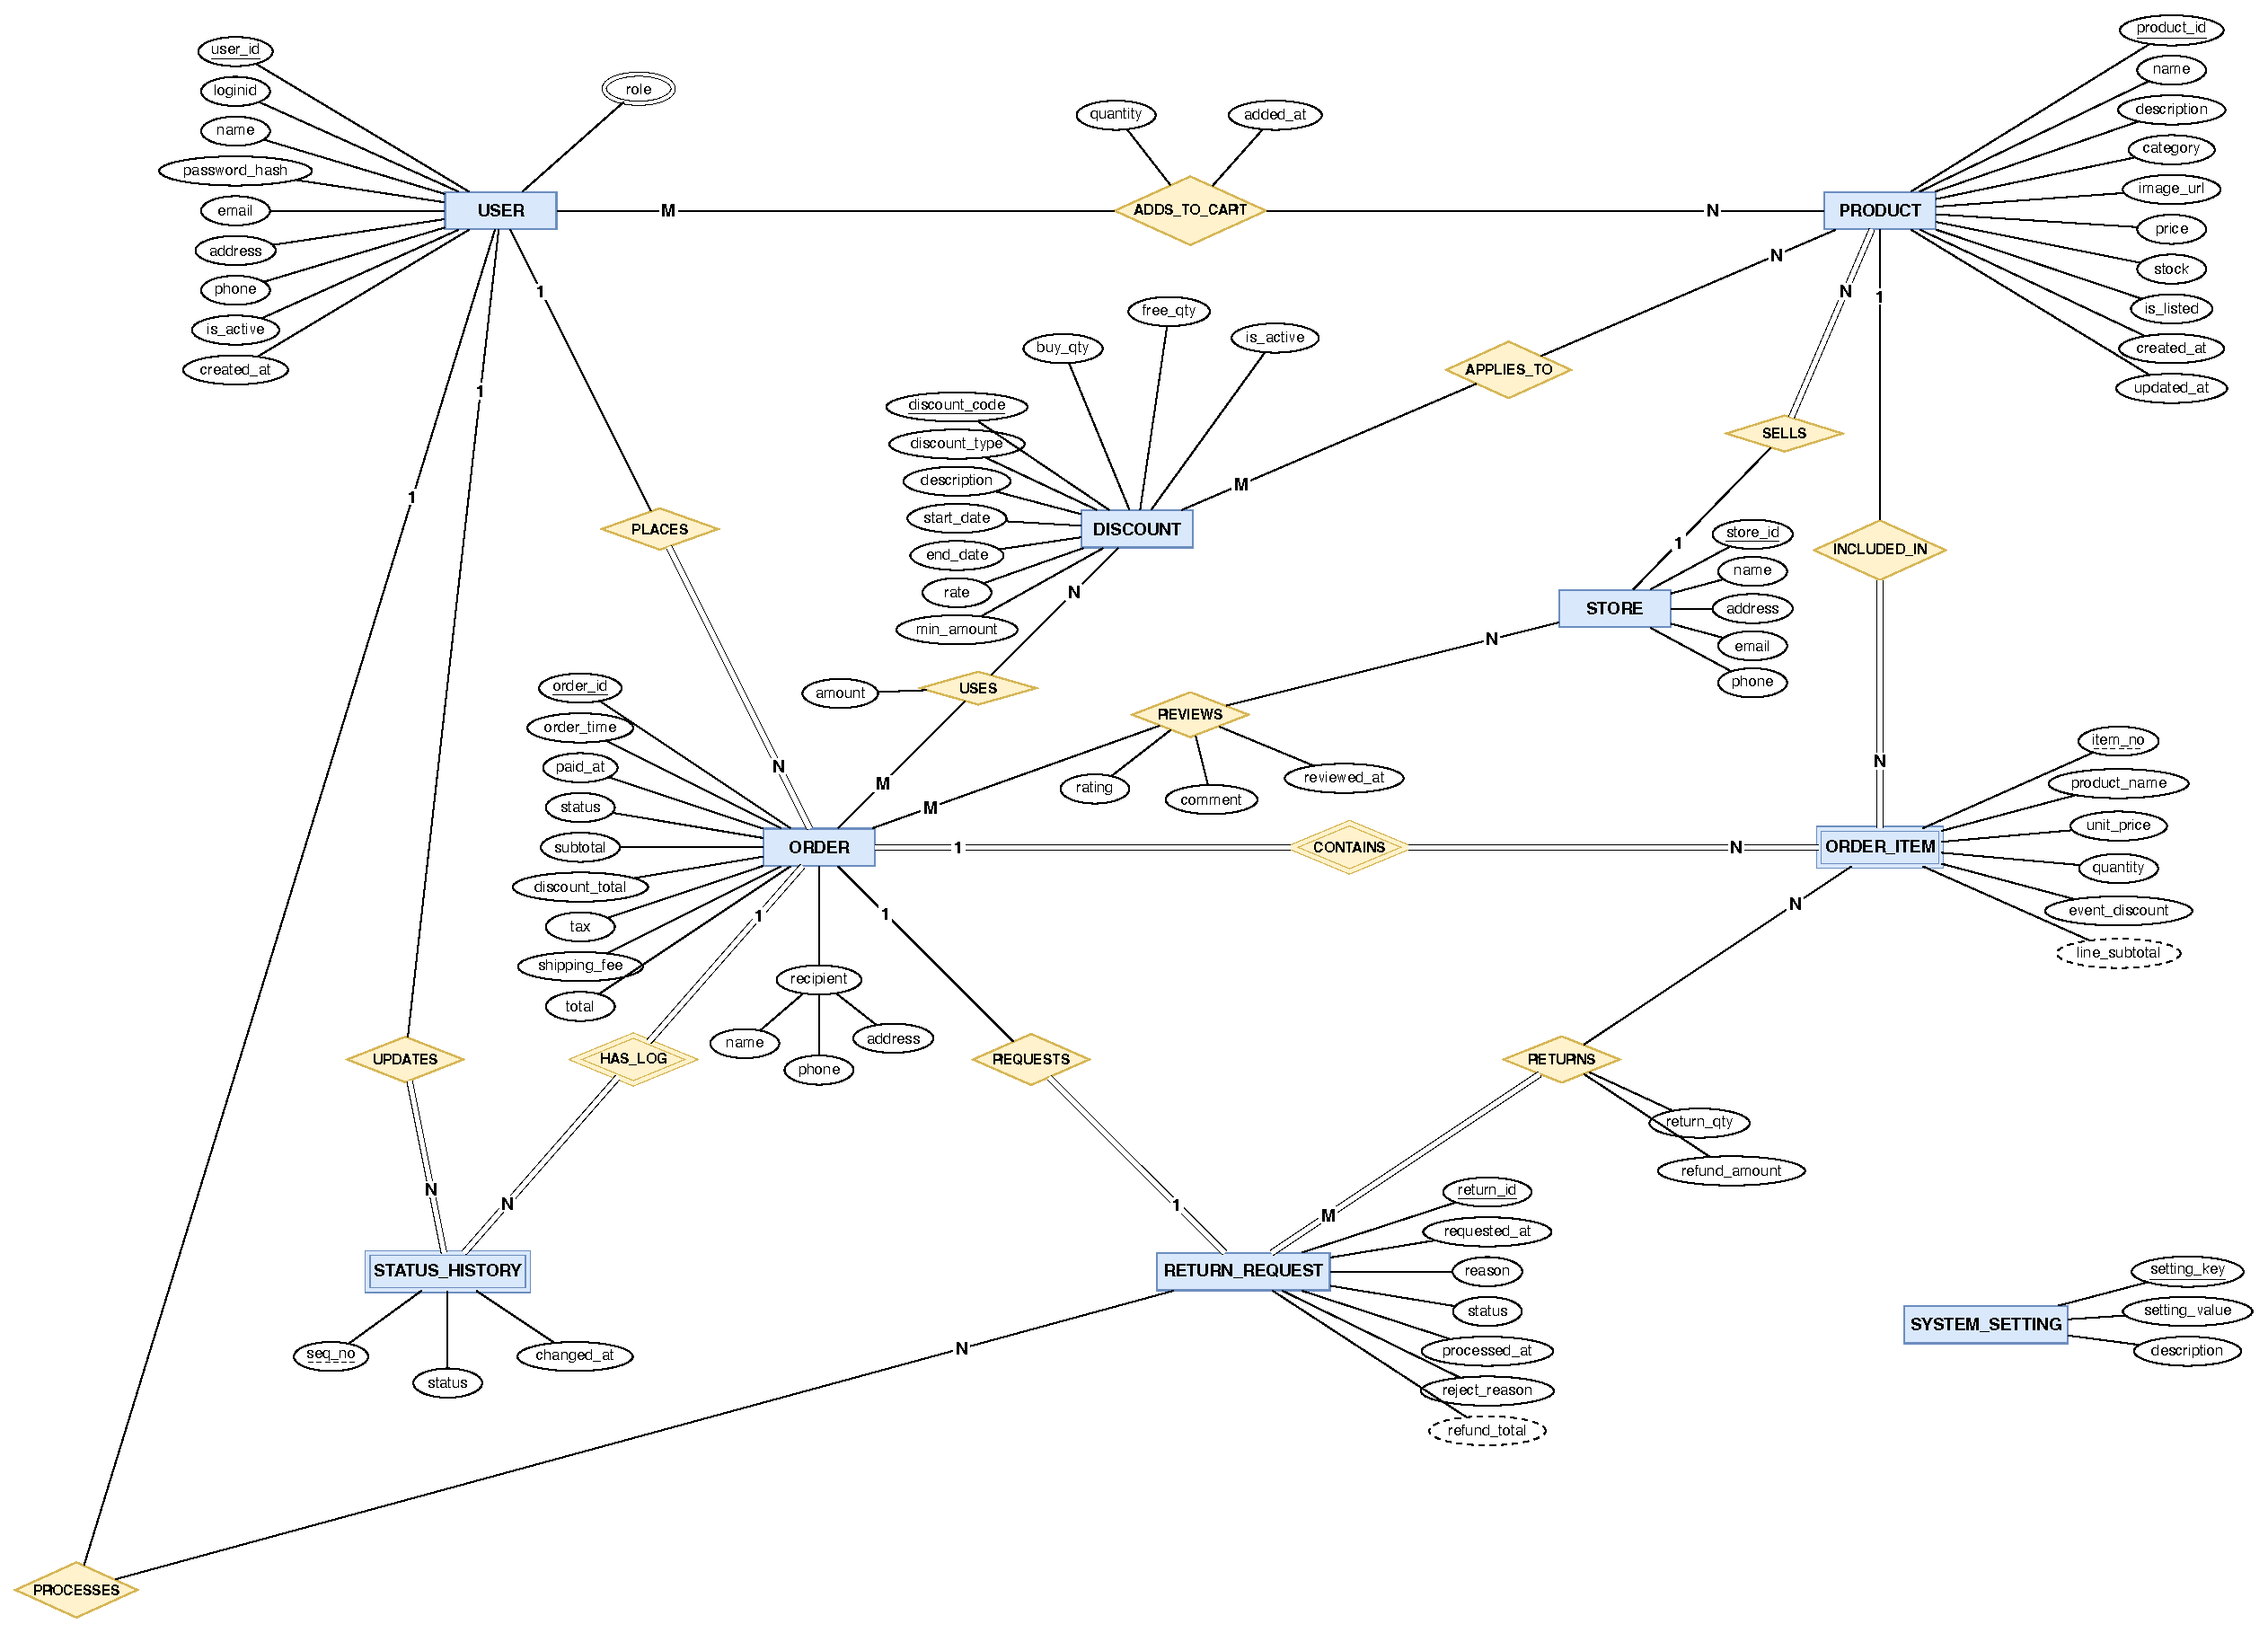
\includegraphics[width=\linewidth,height=0.93\textheight,keepaspectratio]{ER圖/ER_drawio.pdf}
\caption{e-Shop ER Diagram}\label{fig:er}
\end{figure}
\end{landscape}

\subsection{實體說明 (Entities)}

表 \ref{tab:entity} 說明每個實體存放的資料、鍵與屬性。各屬性的資料型態、是否可為 NULL 與限制，列在 4.2 節。

\begingroup\small
\begin{xltabular}{\linewidth}{|>{\raggedright\arraybackslash}p{3.1cm}|>{\raggedright\arraybackslash}X|>{\raggedright\arraybackslash}p{3.2cm}|>{\raggedright\arraybackslash}p{3.6cm}|}
\caption{實體、鍵與屬性}\label{tab:entity}\\
\hline\rowcolor{headgray}\textbf{實體} & \textbf{說明} & \textbf{鍵} & \textbf{屬性}\\\hline\endfirsthead
\hline\rowcolor{headgray}\textbf{實體} & \textbf{說明} & \textbf{鍵} & \textbf{屬性}\\\hline\endhead
USER & 系統所有使用者（顧客、工作人員、平台管理員）。loginid 由使用者自己取，所以另外以系統產生的 user\_id 當主鍵；一位使用者可以有多個角色，所以 role 為多值屬性。 & 主鍵 \at{user_id}；候選鍵 \at{loginid} & loginid、name、password\_hash、email、address、phone、is\_active、created\_at、role（多值）\\\hline
PRODUCT & 商店販售的商品。已被訂單引用的商品不能刪除，只能把 is\_listed 改成 false 下架。 & 主鍵 \at{product_id} & name、description、category、image\_url、price、stock、is\_listed、created\_at、updated\_at\\\hline
DISCOUNT & 折扣政策。三種折扣共用一個實體，以 discount\_type 區分；用不到的規則參數為 NULL。 & 主鍵 \at{discount_code} & discount\_type、description、start\_date、end\_date、rate、min\_amount、buy\_qty、free\_qty、is\_active\\\hline
STORE & 販售商品的商店。 & 主鍵 \at{store_id} & name、address、email、phone\\\hline
ORDER & 顧客確認付款後成立的訂單。金額欄位是付款當下的計算結果，之後折扣或稅率改變也不能變動，所以儲存下來。 & 主鍵 \at{order_id} & order\_time、paid\_at、status、subtotal、discount\_total、tax、shipping\_fee、total、recipient（複合：name、phone、address）\\\hline
ORDER\_ITEM（弱實體） & 訂單中的每一項商品，保存下單當下的品名與單價（BR-08）。離開訂單就沒有意義，所以是 ORDER 的弱實體。 & 部分鍵 \at{item_no}；以 (\at{order_id}, \at{item_no}) 識別 & product\_name、unit\_price、quantity、event\_discount、line\_subtotal（衍生 = unit\_price × quantity）\\\hline
STATUS\_HISTORY（弱實體） & 訂單每一次狀態變更的紀錄（OMS-F-007、OMS-F-008）。 & 部分鍵 \at{seq_no}；以 (\at{order_id}, \at{seq_no}) 識別 & status、changed\_at\\\hline
RETURN\_REQUEST & 顧客提出的退貨申請。 & 主鍵 \at{return_id} & requested\_at、reason、status、processed\_at、reject\_reason、refund\_total（衍生 = 各退貨明細退款金額總和）\\\hline
SYSTEM\_SETTING & 稅率、基本運費等系統參數（BR-22），計算訂單金額時讀取，不和其他實體發生關係。 & 主鍵 \at{setting_key} & setting\_value、description\\\hline
\end{xltabular}
\endgroup

\subsection{關係、基數與參與限制 (Relationships)}

表 \ref{tab:rel} 依 ER 圖由上往下、由左往右的順序列出每個關係。「全部參與」表示該實體的每一筆資料都一定參與這個關係，在 ER 圖中以雙線表示。

\begingroup\small
\begin{xltabular}{\linewidth}{|>{\centering\arraybackslash}p{2.5cm}|>{\centering\arraybackslash}p{3.5cm}|>{\raggedright\arraybackslash}p{3.3cm}|>{\raggedright\arraybackslash}X|}
\caption{關係、基數與參與限制}\label{tab:rel}\\
\hline\rowcolor{headgray}\textbf{關係} & \textbf{實體與基數} & \textbf{參與限制} & \textbf{說明}\\\hline\endfirsthead
\hline\rowcolor{headgray}\textbf{關係} & \textbf{實體與基數} & \textbf{參與限制} & \textbf{說明}\\\hline\endhead
ADDS\_TO\_CART & USER M : N PRODUCT & 兩邊皆部分參與 & 顧客的購物車。關係屬性 quantity（大於 0）、added\_at；同一顧客的同一商品只有一筆（DR-04）。\\\hline
PLACES & USER 1 : N ORDER & ORDER 全部；USER 部分 & 每筆訂單屬於且僅屬於一位顧客（BR-07）；顧客可以沒有訂單，工作人員與管理員也不會下單。\\\hline
APPLIES\_TO & DISCOUNT M : N PRODUCT & 兩邊皆部分參與 & 特殊活動折扣適用的商品。只有 special\_event 類型的折扣會參與，同一商品的期間不得重疊（BR-13）。\\\hline
SELLS & STORE 1 : N PRODUCT & PRODUCT 全部；STORE 部分 & 每個商品屬於且僅屬於一間商店，一間商店可以販售零到多個商品（BR-03）。\\\hline
INCLUDED\_IN & PRODUCT 1 : N ORDER\_ITEM & ORDER\_ITEM 全部；PRODUCT 部分 & 每筆明細對應一個商品，報表依此統計各商品與商店的銷售；商品可以從未被購買。\\\hline
USES & ORDER M : N DISCOUNT & 兩邊皆部分參與 & 訂單實際套用的折扣，關係屬性 amount 為該折扣的折抵金額。三種折扣可同時套用（BR-11）。\\\hline
REVIEWS（選配） & ORDER M : N STORE & 兩邊皆部分參與 & 顧客對已完成訂單中買過的商店評分，關係屬性 rating（1～5）、comment、reviewed\_at；每筆訂單對每間商店最多評一次（BR-24）。\\\hline
CONTAINS（識別關係） & ORDER 1 : N ORDER\_ITEM & 兩邊皆全部參與 & 每筆訂單至少一項明細（BR-07），每筆明細一定屬於一筆訂單；同一訂單中同一商品只有一筆明細。\\\hline
HAS\_LOG（識別關係） & ORDER 1 : N STATUS\_HISTORY & 兩邊皆全部參與 & 訂單成立時就寫入第一筆 received 紀錄，所以每筆訂單至少有一筆歷程。\\\hline
UPDATES & USER 1 : N STATUS\_HISTORY & STATUS\_HISTORY 全部；USER 部分 & 每次狀態變更都記錄操作者：received、cancelled 由顧客觸發，其餘由工作人員更新。\\\hline
REQUESTS & ORDER 1 : 1 RETURN\_REQUEST & RETURN\_REQUEST 全部；ORDER 部分 & 每筆訂單最多只能申請一次退貨（BR-25），所以是 1 : 1。\\\hline
RETURNS & RETURN\_REQUEST M : N ORDER\_ITEM & RETURN\_REQUEST 全部；ORDER\_ITEM 部分 & 退貨申請要退的明細，可以只退部分商品。關係屬性 return\_qty（大於 0 且不超過購買數量）、refund\_amount（核准後依 BR-26 計算）。\\\hline
PROCESSES & USER 1 : N RETURN\_REQUEST & 兩邊皆部分參與 & 處理退貨申請的工作人員；pending 的申請還沒有處理者，所以 RETURN\_REQUEST 是部分參與。\\\hline
\end{xltabular}
\endgroup

\subsection{設計說明}

畫 ER 圖時有幾個地方可以有不同畫法，我們的選擇與理由如下：

\begin{enumerate}
  \item \textbf{角色用多值屬性。}題目說管理員也可以是工作人員，USER 只放一個 role 欄位表示不出來。也可以把顧客、工作人員、管理員畫成三個子類別，但三者的屬性完全一樣，只差在權限，所以用多值屬性 role，轉成資料表就是 \at{user_role}。
  \item \textbf{訂單明細是弱實體。}明細也可以畫成 ORDER 和 PRODUCT 之間的 M:N 關係，但退貨申請要指向「某筆訂單的某一項明細」，關係不能再和其他實體發生關係，所以畫成弱實體 ORDER\_ITEM。
  \item \textbf{特殊活動折扣的期間。}期間屬於 DISCOUNT，但 BR-13 要求同一商品的期間不能重疊，商品和期間要在同一張表才能用資料庫限制檢查，所以轉成資料表時 \at{product_discount} 會複製一份期間，並用複合外鍵確保和 \at{discount} 一致（見 4.3 節）。
  \item \textbf{商店評價連到 ORDER。}BR-24 要求顧客有已完成、且買過該店商品的訂單才能評價，每筆訂單對每間商店只能評一次。畫成 ORDER 和 STORE 的關係，主鍵就是（訂單, 商店），評論者就是訂單的顧客，不用另外存。
  \item \textbf{衍生屬性。}明細小計與退款總額可以直接算出，不另外儲存；訂單的金額欄位雖然也算得出來，但它們是付款當下的結果，必須保留，所以仍然儲存。
\end{enumerate}

\subsection{ER 圖無法表示的限制}

以下規則畫不進 ER 圖，4.3 節說明在資料庫中如何實作：

\begin{itemize}
  \item 只有具有 customer 角色的使用者能參與 PLACES 與 ADDS\_TO\_CART；只有 staff 能參與 PROCESSES（BR-21）。
  \item 購買數量不得超過商品目前的庫存，庫存不得為負數（BR-06）。
  \item 只有 special\_event 類型的折扣能參與 APPLIES\_TO，且同一商品的期間不能重疊（BR-13）。
  \item 訂單狀態只能依 received → processing → shipping → closed 前進；cancelled 只能從 received 變過去（BR-19）。
  \item 退貨數量不得超過購買數量；只有 processing、shipping、closed 的訂單可以申請退貨（BR-25）。
\end{itemize}

% ================= Section 4 =================
\clearpage
\section{邏輯資料庫綱要 (Logic Database Schema)}

\subsection{Schema of the Database}

我們依 ER-to-Relational mapping 的步驟把 ER 圖轉成 15 張資料表：一般實體各成一張表（複合屬性 recipient 拆成三個欄位，衍生屬性不建欄位）；弱實體的主鍵為擁有者主鍵加部分鍵；1:1 的 REQUESTS 把外鍵放在全部參與的 \at{return_request} 並設為 UNIQUE；1:N 關係在 N 端加外鍵；M:N 關係與多值屬性 role 各自成表。因為 user 與 order 是 SQL 保留字，這兩張表命名為 \at{users} 與 \at{orders}。

圖 \ref{fig:schema} 為 schema 圖，箭頭由外鍵欄位指向被參照的主鍵欄位，底線為主鍵，標 (FK) 為外鍵；複合外鍵只從第一個欄位畫一條箭頭。

\begin{landscape}
\begin{figure}[p]
\centering
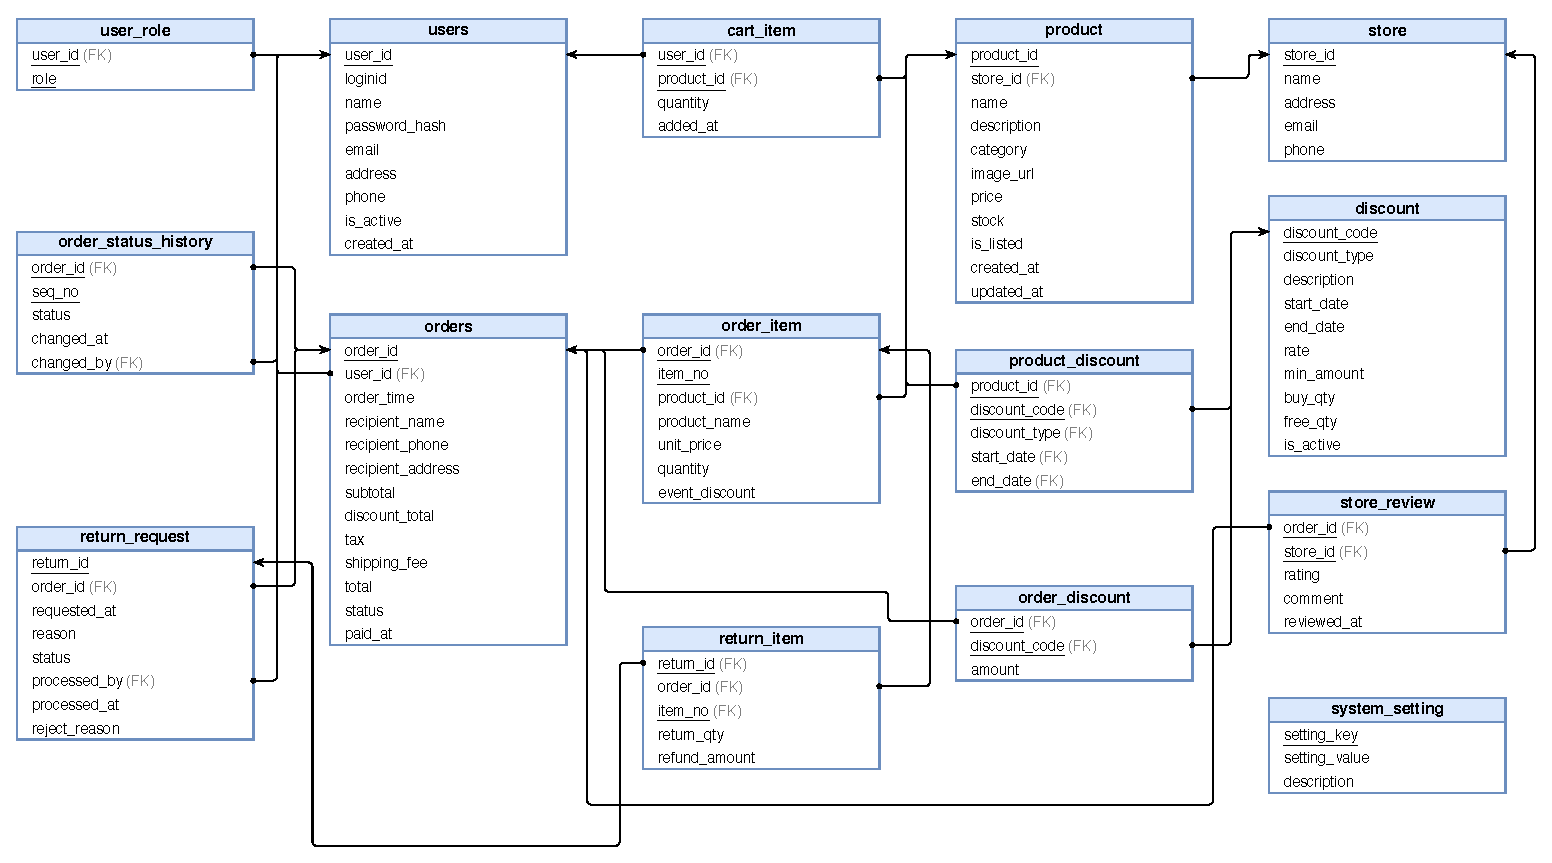
\includegraphics[width=\linewidth,height=0.9\textheight,keepaspectratio]{schema圖/schema_diagram.pdf}
\caption{e-Shop Schema Diagram}\label{fig:schema}
\end{figure}
\end{landscape}

\subsection{Domain of the Database}

以下列出每張資料表的欄位。金額一律以新台幣「元」為單位，用 \at{NUMERIC(10,0)} 存整數；折扣率用 \at{NUMERIC(4,3)}；編號類主鍵用 \at{SERIAL}（自動遞增整數）。Key 欄的 PK 為主鍵、FK 為外鍵。

\begin{domtable}{USERS}{存放所有使用者的帳號資料}
\dr{user_id}{SERIAL}{PK}{Not null}{使用者編號}
\dr{loginid}{VARCHAR(30)}{Unique}{Not null}{登入帳號，不可重複（BR-01）}
\dr{name}{VARCHAR(50)}{}{Not null}{姓名}
\dr{password_hash}{VARCHAR(100)}{}{Not null}{bcrypt 雜湊後的密碼}
\dr{email}{VARCHAR(100)}{}{Not null}{電子郵件}
\dr{address}{VARCHAR(200)}{}{}{地址}
\dr{phone}{VARCHAR(20)}{}{}{電話}
\dr{is_active}{BOOLEAN}{}{Not null}{帳號是否啟用，預設 TRUE}
\dr{created_at}{TIMESTAMP}{}{Not null}{建立時間，預設 now()}
\end{domtable}

\begin{domtable}{USER\_ROLE}{存放使用者的角色，一位使用者可以有多個角色}
\dr{user_id}{INT}{PK, FK}{Not null}{使用者編號 Reference (USERS)，ON DELETE CASCADE}
\dr{role}{VARCHAR(10)}{PK}{Not null}{角色，只能是 customer、staff、admin}
\end{domtable}

\begin{domtable}{STORE}{存放商店資料}
\dr{store_id}{SERIAL}{PK}{Not null}{商店編號}
\dr{name}{VARCHAR(50)}{}{Not null}{商店名稱}
\dr{address}{VARCHAR(200)}{}{Not null}{商店地址}
\dr{email}{VARCHAR(100)}{}{Not null}{聯絡 Email}
\dr{phone}{VARCHAR(20)}{}{Not null}{聯絡電話}
\end{domtable}

\begin{domtable}{PRODUCT}{存放商品資料}
\dr{product_id}{SERIAL}{PK}{Not null}{商品編號}
\dr{store_id}{INT}{FK}{Not null}{所屬商店 Reference (STORE)}
\dr{name}{VARCHAR(100)}{}{Not null}{商品名稱}
\dr{description}{TEXT}{}{}{商品描述}
\dr{category}{VARCHAR(30)}{}{}{分類}
\dr{image_url}{VARCHAR(300)}{}{}{商品圖片網址}
\dr{price}{NUMERIC(10,0)}{}{Not null}{售價（price > 0）}
\dr{stock}{INT}{}{Not null}{庫存數量（stock >= 0）}
\dr{is_listed}{BOOLEAN}{}{Not null}{是否上架，預設 TRUE}
\dr{created_at}{TIMESTAMP}{}{Not null}{上架時間}
\dr{updated_at}{TIMESTAMP}{}{Not null}{最後修改時間}
\end{domtable}

\begin{domtable}{CART\_ITEM}{存放顧客購物車中的商品}
\dr{user_id}{INT}{PK, FK}{Not null}{顧客編號 Reference (USERS)，ON DELETE CASCADE}
\dr{product_id}{INT}{PK, FK}{Not null}{商品編號 Reference (PRODUCT)，ON DELETE CASCADE}
\dr{quantity}{INT}{}{Not null}{數量（quantity > 0）}
\dr{added_at}{TIMESTAMP}{}{Not null}{加入時間}
\end{domtable}

\begin{domtable}{ORDERS}{存放訂單資料}
\dr{order_id}{SERIAL}{PK}{Not null}{訂單編號}
\dr{user_id}{INT}{FK}{Not null}{下單顧客 Reference (USERS)}
\dr{order_time}{TIMESTAMP}{}{Not null}{下單時間}
\dr{recipient_name}{VARCHAR(50)}{}{Not null}{收件人姓名}
\dr{recipient_phone}{VARCHAR(20)}{}{Not null}{收件人電話}
\dr{recipient_address}{VARCHAR(200)}{}{Not null}{收件地址}
\dr{subtotal}{NUMERIC(10,0)}{}{Not null}{商品小計（>= 0）}
\dr{discount_total}{NUMERIC(10,0)}{}{Not null}{折扣總額（>= 0），預設 0}
\dr{tax}{NUMERIC(10,0)}{}{Not null}{稅額（>= 0）}
\dr{shipping_fee}{NUMERIC(10,0)}{}{Not null}{運費（>= 0）}
\dr{total}{NUMERIC(10,0)}{}{Not null}{訂單總額（>= 0），計算方式見 BR-09、BR-10}
\dr{status}{VARCHAR(10)}{}{Not null}{訂單狀態：received、processing、shipping、closed、cancelled、returned，預設 received}
\dr{paid_at}{TIMESTAMP}{}{Not null}{確認付款時間}
\end{domtable}

\begin{domtable}{ORDER\_ITEM}{存放訂單明細；(order\_id, product\_id) 為 UNIQUE}
\dr{order_id}{INT}{PK, FK}{Not null}{訂單編號 Reference (ORDERS)，ON DELETE CASCADE}
\dr{item_no}{SMALLINT}{PK}{Not null}{明細序號（> 0）}
\dr{product_id}{INT}{FK}{Not null}{商品編號 Reference (PRODUCT)}
\dr{product_name}{VARCHAR(100)}{}{Not null}{下單當下的品名}
\dr{unit_price}{NUMERIC(10,0)}{}{Not null}{下單當下的單價（> 0）}
\dr{quantity}{INT}{}{Not null}{購買數量（> 0）}
\dr{event_discount}{NUMERIC(10,0)}{}{Not null}{特殊活動折抵金額，介於 0 與 unit\_price × quantity 之間，預設 0}
\end{domtable}

\begin{domtable}{ORDER\_STATUS\_HISTORY}{存放訂單狀態變更紀錄}
\dr{order_id}{INT}{PK, FK}{Not null}{訂單編號 Reference (ORDERS)，ON DELETE CASCADE}
\dr{seq_no}{SMALLINT}{PK}{Not null}{變更序號（> 0）}
\dr{status}{VARCHAR(10)}{}{Not null}{變更後的狀態（同 ORDERS.status 的六種）}
\dr{changed_at}{TIMESTAMP}{}{Not null}{變更時間}
\dr{changed_by}{INT}{FK}{Not null}{操作者 Reference (USERS)}
\end{domtable}

\begin{domtable}{DISCOUNT}{存放折扣政策；另有表格層級 CHECK 依類型限制規則參數（BR-17）}
\dr{discount_code}{VARCHAR(20)}{PK}{Not null}{折扣代碼，由系統產生}
\dr{discount_type}{VARCHAR(15)}{}{Not null}{shipping、seasonal、special\_event}
\dr{description}{VARCHAR(200)}{}{Not null}{折扣說明}
\dr{start_date}{DATE}{}{Not null}{開始日期（start\_date <= end\_date）}
\dr{end_date}{DATE}{}{Not null}{結束日期}
\dr{rate}{NUMERIC(4,3)}{}{}{折扣率（0 < rate < 1）}
\dr{min_amount}{NUMERIC(10,0)}{}{}{運費折扣門檻（> 0）}
\dr{buy_qty}{SMALLINT}{}{}{買 X 送 Y 的 X（> 0）}
\dr{free_qty}{SMALLINT}{}{}{買 X 送 Y 的 Y（> 0），與 buy\_qty 同時有值或同時為 NULL}
\dr{is_active}{BOOLEAN}{}{Not null}{是否啟用，預設 TRUE}
\end{domtable}
表格層級 CHECK 的內容：shipping 只能有 min\_amount；seasonal 只能有 rate；special\_event 必須在 rate 與 buy\_qty／free\_qty 之中剛好選一種。另外 (discount\_code, discount\_type, start\_date, end\_date) 設為 UNIQUE，給 PRODUCT\_DISCOUNT 的複合外鍵使用。

\begin{domtable}{PRODUCT\_DISCOUNT}{存放特殊活動折扣適用的商品}
\dr{product_id}{INT}{PK, FK}{Not null}{商品編號 Reference (PRODUCT)，ON DELETE CASCADE}
\dr{discount_code}{VARCHAR(20)}{PK, FK}{Not null}{折扣代碼}
\dr{discount_type}{VARCHAR(15)}{FK}{Not null}{只能是 special\_event}
\dr{start_date}{DATE}{FK}{Not null}{折扣開始日期}
\dr{end_date}{DATE}{FK}{Not null}{折扣結束日期}
\end{domtable}
(discount\_code, discount\_type, start\_date, end\_date) 為複合外鍵 Reference (DISCOUNT)，ON UPDATE CASCADE、ON DELETE CASCADE；並有 EXCLUDE 限制防止同一商品的期間重疊（見 4.3 節）。

\begin{domtable}{ORDER\_DISCOUNT}{存放訂單實際套用的折扣}
\dr{order_id}{INT}{PK, FK}{Not null}{訂單編號 Reference (ORDERS)，ON DELETE CASCADE}
\dr{discount_code}{VARCHAR(20)}{PK, FK}{Not null}{折扣代碼 Reference (DISCOUNT)}
\dr{amount}{NUMERIC(10,0)}{}{Not null}{該折扣的折抵金額（>= 0）}
\end{domtable}

\begin{domtable}{RETURN\_REQUEST}{存放退貨申請；(return\_id, order\_id) 為 UNIQUE，給 RETURN\_ITEM 的複合外鍵使用}
\dr{return_id}{SERIAL}{PK}{Not null}{退貨申請編號}
\dr{order_id}{INT}{FK, Unique}{Not null}{訂單編號 Reference (ORDERS)；每筆訂單只能申請一次}
\dr{requested_at}{TIMESTAMP}{}{Not null}{申請時間}
\dr{reason}{VARCHAR(300)}{}{Not null}{退貨原因}
\dr{status}{VARCHAR(10)}{}{Not null}{pending、approved、rejected，預設 pending}
\dr{processed_by}{INT}{FK}{}{處理的工作人員 Reference (USERS)；pending 時為 NULL}
\dr{processed_at}{TIMESTAMP}{}{}{處理時間；pending 時為 NULL}
\dr{reject_reason}{VARCHAR(300)}{}{}{拒絕原因；只有 rejected 時必須填寫}
\end{domtable}

\begin{domtable}{RETURN\_ITEM}{存放退貨申請要退的明細}
\dr{return_id}{INT}{PK, FK}{Not null}{退貨申請編號；(return\_id, order\_id) Reference (RETURN\_REQUEST)}
\dr{order_id}{INT}{FK}{Not null}{訂單編號；確保退的明細屬於同一筆訂單}
\dr{item_no}{SMALLINT}{PK, FK}{Not null}{明細序號；(order\_id, item\_no) Reference (ORDER\_ITEM)}
\dr{return_qty}{INT}{}{Not null}{退貨數量（> 0）}
\dr{refund_amount}{NUMERIC(10,0)}{}{}{該項退款金額（>= 0），核准前為 NULL}
\end{domtable}

\begin{domtable}{STORE\_REVIEW}{存放商店評價（選配）}
\dr{order_id}{INT}{PK, FK}{Not null}{訂單編號 Reference (ORDERS)}
\dr{store_id}{INT}{PK, FK}{Not null}{商店編號 Reference (STORE)}
\dr{rating}{SMALLINT}{}{Not null}{評分（1 至 5）}
\dr{comment}{VARCHAR(500)}{}{}{評論內容}
\dr{reviewed_at}{TIMESTAMP}{}{Not null}{評價時間}
\end{domtable}

\begin{domtable}{SYSTEM\_SETTING}{存放系統參數，例如 tax\_rate = 0.05、base\_shipping\_fee = 100}
\dr{setting_key}{VARCHAR(30)}{PK}{Not null}{參數名稱}
\dr{setting_value}{VARCHAR(50)}{}{Not null}{參數值}
\dr{description}{VARCHAR(100)}{}{}{參數說明}
\end{domtable}

\subsection{完整性限制的實作}

\textbf{參考完整性。}外鍵預設為 NO ACTION，被參照的資料不能直接刪除。例如商品已出現在訂單明細中就刪不掉，只能把 is\_listed 改成 false；用過的折扣與有訂單的顧客也一樣，符合 BR-20。只有「跟著主體一起消失也沒關係」的資料設定 ON DELETE CASCADE，例如使用者的角色與購物車、商品的購物車項目與折扣設定、訂單的明細與狀態歷程。

\textbf{特殊活動折扣期間不重疊（BR-13）。}做法分三步：(1) \at{product_discount} 存一份期間，用複合外鍵參照 \at{discount}，期間一定和折扣政策相同，修改折扣期間時 ON UPDATE CASCADE 會自動同步；(2) \at{discount_type} 以 CHECK 限定為 special\_event，運費與季節性折扣掛不到商品上；(3) 使用 PostgreSQL 的 EXCLUDE 限制，讓同一個 product\_id 的兩筆資料期間（含首尾兩日）不能有交集：
\begin{Verbatim}[fontsize=\small,xleftmargin=2em]
EXCLUDE USING gist (product_id WITH =,
                    daterange(start_date, end_date, '[]') WITH &&)
\end{Verbatim}

\textbf{以 CHECK 與 UNIQUE 處理的規則。}BR-01、BR-04、BR-05、BR-14、BR-15、BR-17、BR-19 的狀態值範圍、BR-24 的評分範圍與每單每店一則評價、BR-25 的每筆訂單只能申請一次退貨，都已寫在 4.2 節的欄位限制中。我們把 schema 寫成 SQL（Appendix）並在 PostgreSQL 上實際建立，用故意違規的資料測試（重複的 loginid、數量為 0、庫存扣成負數、期間重疊、不合法的狀態、同一訂單第二次申請退貨、退別張訂單的明細等），資料庫都會拒絕。

\textbf{需要在交易或 trigger 中處理的規則。}以下規則牽涉其他資料表或狀態的前後順序，預計在 Phase 3 以 trigger 或後端交易實作：

\begingroup\small
\begin{xltabular}{\linewidth}{|>{\centering\arraybackslash}p{1.6cm}|>{\raggedright\arraybackslash}X|>{\raggedright\arraybackslash}p{5.2cm}|}
\caption{需要 trigger 或交易處理的規則}\\
\hline\rowcolor{headgray}\textbf{規則} & \textbf{內容} & \textbf{預計做法}\\\hline\endfirsthead
\hline\rowcolor{headgray}\textbf{規則} & \textbf{內容} & \textbf{預計做法}\\\hline\endhead
BR-02 & 至少保留一位啟用中的平台管理員 & user\_role 的 BEFORE DELETE 與 users 的 BEFORE UPDATE trigger 檢查移除角色或停用帳號後仍有啟用中的 admin\\\hline
BR-06 & 購買數量不得超過庫存 & 結帳交易中以 SELECT … FOR UPDATE 鎖定商品再扣庫存；stock >= 0 的 CHECK 是最後一道防線\\\hline
BR-07 & 每筆訂單至少一項明細 & 結帳交易中一起寫入訂單與明細\\\hline
BR-19 & 狀態只能依序前進 & orders 的 BEFORE UPDATE trigger 比對新舊狀態，並自動寫入 order\_status\_history\\\hline
BR-21 & 只有顧客能下單、只有工作人員能處理退貨 & trigger 檢查 user\_role，後端 API 也會檢查\\\hline
BR-24 & 只能評價已完成且買過該店商品的訂單 & store\_review 的 BEFORE INSERT trigger\\\hline
BR-25 & 退貨數量不超過購買數量；只有特定狀態的訂單能申請 & return\_request、return\_item 的 BEFORE INSERT trigger\\\hline
\end{xltabular}
\endgroup


\clearpage
% ================= Glossary =================
\section*{Glossary}
\addcontentsline{toc}{section}{Glossary}

\begin{xltabular}{\linewidth}{|>{\centering\arraybackslash}p{3.4cm}|X|}
\hline\rowcolor{headgray}\textbf{名詞} & \textbf{說明}\\\hline\endhead
SRS & Software Requirements Specification，系統需求規格書。\\\hline
SPA & Single Page Application，單頁式網頁應用程式。\\\hline
REST API & 以 HTTP 方法（GET、POST、PUT、DELETE）操作資源的網路應用程式介面。\\\hline
JSON & JavaScript Object Notation，前後端交換資料使用的格式。\\\hline
JWT & JSON Web Token，登入後用來識別使用者身分的權杖。\\\hline
bcrypt & 一種加鹽的密碼雜湊演算法。\\\hline
ORM & Object-Relational Mapping，以物件操作關聯式資料庫的技術，本系統使用 SQLAlchemy。\\\hline
CRUD & Create、Read、Update、Delete，新增、查詢、修改、刪除。\\\hline
ER Model & Entity-Relationship Model，以實體、屬性與關係描述資料的概念模型。\\\hline
弱實體 (Weak Entity) & 沒有自己的鍵、必須依附擁有者實體才能識別的實體，本系統為 ORDER\_ITEM 與 STATUS\_HISTORY。\\\hline
部分鍵 (Partial Key) & 弱實體中與擁有者主鍵一起識別每筆資料的屬性。\\\hline
基數比 (Cardinality Ratio) & 一個實體可以和另一實體的幾筆資料發生關係，例如 1:1、1:N、M:N。\\\hline
參與限制 (Participation) & 實體是否每一筆都必須參與某個關係，分為全部參與與部分參與。\\\hline
候選鍵 (Candidate Key) & 可以唯一識別每筆資料、但沒有被選為主鍵的屬性，例如 loginid。\\\hline
EXCLUDE 約束 & PostgreSQL 的限制，可以規定任兩筆資料在指定欄位上不能同時「相等且期間重疊」。\\\hline
主鍵 (PK) & Primary Key，唯一識別資料表中每一筆資料的屬性。\\\hline
外鍵 (FK) & Foreign Key，參照其他資料表主鍵的屬性，用以維持參考完整性。\\\hline
交易 (Transaction) & 一組必須全部成功或全部失敗的資料庫操作。\\\hline
運費折扣 & 訂單金額達門檻時免運費的折扣，作用於整筆訂單。\\\hline
季節性折扣 & 指定期間內依折扣率折抵整筆訂單金額的折扣。\\\hline
特殊活動折扣 & 指定期間內作用於指定商品的折扣，規則為折扣率或買 X 送 Y。\\\hline
折扣代碼 & 系統指派給每個折扣政策的唯一代碼。\\\hline
received & 訂單已送出，系統已接收。\\\hline
processing & 工作人員處理中。\\\hline
shipping & 已出貨，配送中。\\\hline
closed & 訂單已完成。\\\hline
cancelled & 訂單在 received 狀態時由顧客取消。\\\hline
returned & 訂單所有商品的退貨申請都經工作人員核准，訂單已全部退貨。\\\hline
退貨申請 & 顧客對已處理、已出貨或已完成的訂單提出的退貨要求，可以只退部分商品，須經工作人員同意；每筆訂單限申請一次。\\\hline
RWD & Responsive Web Design，響應式網頁設計。\\\hline
\end{xltabular}

\clearpage
% ================= References =================
\section*{References}
\addcontentsline{toc}{section}{References}

\begin{enumerate}[label={[\arabic*]},leftmargin=2.5em,itemsep=0.4em]
  \item 國立臺北科技大學資訊工程系，資料庫系統課程專題說明（e-Shop Project Descriptions），2026。
  \item 國立臺北科技大學資訊工程系，系統需求規格書範本（SRS.docx）。
  \item NTUT Software Engineering Lab, Database System Example Project. \url{https://github.com/ntutselab/Database-System-Example-Project}
  \item R. Elmasri and S. B. Navathe, \textit{Fundamentals of Database Systems}, 7th ed., Pearson, 2016.
  \item IEEE Std 830-1998, IEEE Recommended Practice for Software Requirements Specifications.
  \item PostgreSQL Global Development Group, PostgreSQL 16 Documentation. \url{https://www.postgresql.org/docs/16/}
  \item FastAPI Documentation. \url{https://fastapi.tiangolo.com/}
  \item SQLAlchemy Documentation. \url{https://docs.sqlalchemy.org/}
  \item React Documentation. \url{https://react.dev/}
\end{enumerate}

\clearpage
% ================= Appendix =================
\section*{Appendix}
\addcontentsline{toc}{section}{Appendix}

以下是依 Section 4 寫成的 PostgreSQL DDL（\at{schema.sql}），已在 PostgreSQL 上成功執行。Phase 3 會再加上 trigger 與初始資料。

\VerbatimInput[fontsize=\scriptsize,numbers=left,numbersep=4pt]{schema.sql}

\end{document}
